%------------------------------
\chapter{Architektúra}
%------------------------------

A fejlesztés során elsődleges célom volt, hogy egy olyan architektúrára alapozzam az alkalmazást, mely megfelelően szétválasztja a felelősségeket, és ezáltal egy könnyen karbantartható, átlátható kódot alkossak. Először egyből az MVVM (Model - View - ViewModel) architektúrára gondoltam, mivel azt már korábban is használtam, és jó tapasztalataim voltak vele, aztán amikor erről beszélgettem a konzulensemmel, akkor ő a RainbowCake-et\cite{Rainbowcake} ajánlotta. Egy MVVM-re építő architektúráról van szó, melynek fő fókusza a felelősségek szétválasztása és a képernyő konzisztens állapotban tartása. Tekintve, hogy ez pontosan megegyezik a céljaimmal, így a kipróbálása mellett döntöttem.

\section{Felépítés}

Az architektúra rétegeit a \refstruc{fig:RainbowCakeLayers} szemlélteti.

\begin{figure}[!ht]
	\centering
	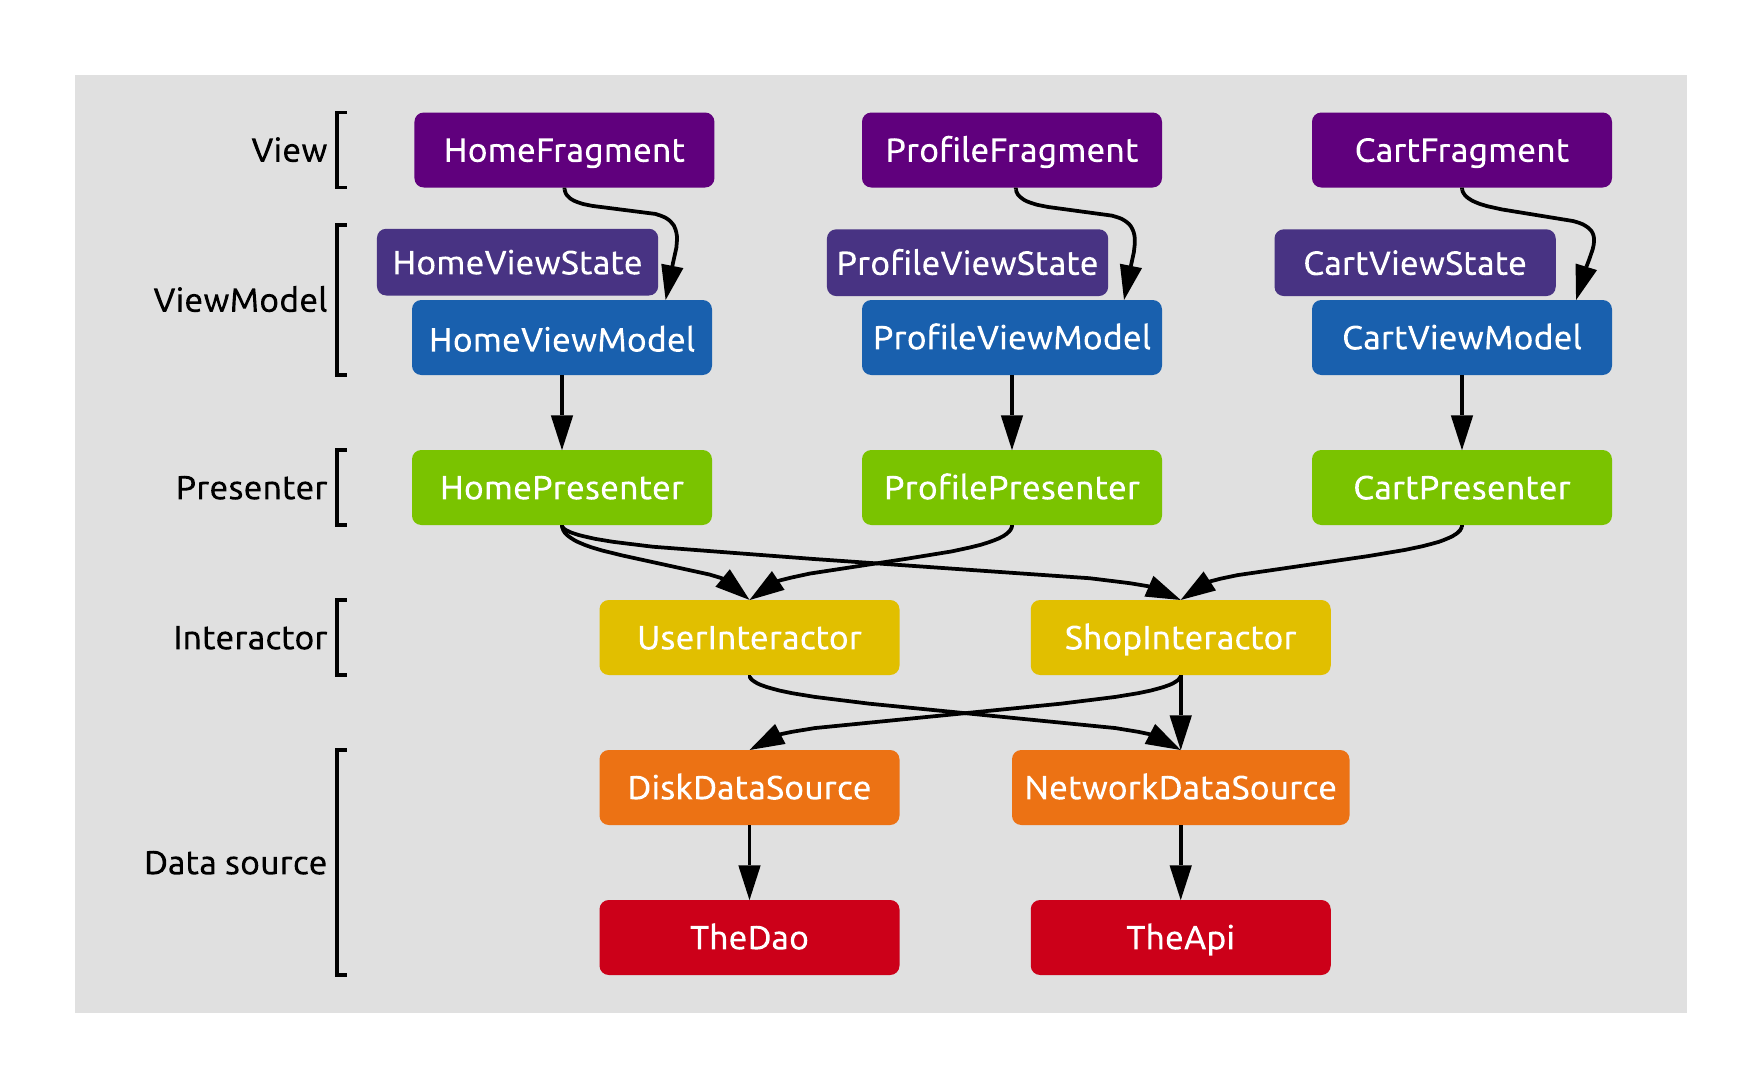
\includegraphics[width=150mm, keepaspectratio]{figures/final-architecture.png}
	\caption{A RainbowCake architektúra rétegei.}
	\label{fig:RainbowCakeLayers}
\end{figure}

\subsection{View}
A view-k alkotják az alkalmazás képernyőit, melyekkel a felhasználó találkozik használat közben. Ezek lehetnek Activityk vagy Fragmentek, és fő feladatuk továbbítani a felhasználói inputot a ViewModel felé, melytől cserébe új adatot, állapotot vagy eseményt kapnak. 

\subsection{ViewModel}
A felhasználói felülettel kapcsolatos logikát végzik, illetve tárolják és a Presentertől kapott adatok alapján frissítik a képernyőhöz tartozó ViewState-et.

\subsection{Presenter}
Háttérszálra teszik a hívásokat, és továbbítják azokat az Interactorok felé, majd az eredményt képernyő specifikus prezentációs modellekké transzformálják, és azt adják oda a ViewModelnek. A projektből ezt a réteget teljesen kihagytam, mivel ugyanazt a modellt jeleníti meg, mint amit az adatbázisból visszakap, így nem volt szükség a modelltranszformációra. 

\subsection{Interactor}
Az Interactorok, ahogy az ábrán is látható, nem egy-egy képernyőhöz köthetők, hanem funkcionalitásokhoz. Ők végzik a fő üzleti logikát, manipulálják az adatokat és számításokat végeznek. Az alkalmazásomban csak egyetlen darab van, ugyanis az adatok megjelenítése nem igényel sok üzleti logikát, viszont Presenterek hiányában ő kapta meg a felelősséget, hogy a hívásokat háttérszálra tegye. 

\subsection{DataSource}
Egységes interfészt biztosítanak az adathozzáféréshez, feladatuk a különböző hívások (pl.: lokális adatbázis, Firebase) implementációjának elfedése, és az adatok konzisztens állapotban tartása. 

\section{Funkciók}

A következőkben röviden kifejtem az architektúra főbb funkcióit, melyek segítségemre voltak az alkalmazás fejlesztése során. 

\subsection{Dependency Injection}
A függőséginjektálás - dependency injection, röviden DI - egy gyakran használt technika, mely jelentősen könnyebbé teszi a kód újrafelhasználását, refaktorálását és tesztelését.\cite{DepInjection}

Függőségnek nevezzük azt, amikor egy osztálynak szüksége van egy másik osztály referenciájára. Ilyenkor, ha ezt saját maga példányosítja, akkor szoros csatolás jön létre a két osztály között, ennek következményeképpen pedig nem lehet a tartalmazott objektum helyett később egy másik implementációt vagy leszármazottat használni. Emellett a tesztelés is megnehezedik, hiszen az osztály egy valódi példányt használ a másikból, azt nem tudjuk egy tesztobjektummal helyettesíteni.

Függőséginjektálásról akkor beszélünk, hogyha a fent leírt módszer helyett az osztály a függőségeit paraméterként kapja, például a konstruktorban. Ezáltal az említett problémák megszűnnek, az osztályunk újrafelhasználható lesz, és könnyedén tesztelni is tudjuk, ha valós függőség helyett egy mock objektumot adunk neki. 

A DI megvalósítására két opció létezik: manuális, illetve automatizált. Az előbbi kisebb alkalmazásoknál megoldható lehet, ha csak pár osztály létezik kevés függőséggel, de nagyon hamar kezelhetetlenné válik az alkalmazás növekedésével. Erre nyújtanak megoldást a különböző könyvtárak, melyek megfelelő beállítások mellett automatikusan elvégzik a függőségek létrehozását és biztosítását. 
Egy ilyen könyvtár a Dagger 2, mely az egyik legnépszerűbb ezen a téren. A RainbowCake beépítetten támogatja a használatát, csak a megfelelő függőségeket kell felvenni a projektbe. Ezt követően még pár beállítást el kell végeznünk a projekten, majd az injektálni kívánt konstruktorokat \emph{@Inject} annotációval megjelölni, a többit pedig elvégzi helyettünk.

\subsection{View State}
A RainbowCake állapotkezelése jelentősen megkönnyíti a UI különböző állapotainak nyomon követését, és az annak megfelelő nézet megjelenítését. Ha egy képernyőnek több egymástól független, elkülöníthető állapota van, akkor ezt nem érdemes egyetlen \emph{data class} tagváltozóiban tárolni, mert az inkonzisztens állapothoz vezethet.\cite{ViewState} 

Erre kínál egy kényelmes megoldást a Kotlinban elérhető \emph{sealed class}, mely egy olyan osztály, aminek fordítási időben ismerjük az összes leszármazottját. Ha a fragment állapotait egy ilyen \emph{sealed class}-ból származtatjuk le, akkor lévén osztályok, tartalmazhatnak saját tagváltozókat (például a megjelenítendő adatokat vagy a hibaüzenetet), és a Kotlin \emph{when} feltételes szerkezetének segítségével ki lehet kényszeríteni, hogy minden állapot le legyen kezelve. 

Így már nem fordulhat elő inkonzisztencia, hiszen az egymást kölcsönösen kizáró állapotokból egyszerre csak egy lehet aktív a futás során. A képernyő render logikája pedig leegyszerűsödik: az architektúra által biztosított \emph{render} függvényben az állapottól függően változtathatjuk a megjelenítést. Az pedig garantálva van, hogy a \emph{render} mindig lefut, amikor megváltozik a képernyő állapota. 

\subsection{ViewFlipper}
A ViewFlipper egy layout komponens, mely az állapotok olvasható elkülönítését teszi lehetővé. \cite{ViewFlipper} Ugyanis ha a képernyő minden elemét külön manipuláljuk a fent említett \emph{render} függvényben, akkor ez egy idő után olvashatatlan kódot fog eredményezni, rengeteg hibalehetőséggel. Ezt orvosolja a ViewFlipper, melyben egyszerre egy tartalmazott layoutot tudunk megjeleníteni, így nem kell manuálisan állítani a külön elemek láthatóságát. Használata rendkívül egyszerű, a layoutot leíró XML fájlban egy ViewFlipper komponenst kell létrehozni (\refstruc{fig:ViewFlipperComponent}), az épp látható gyerek elemét pedig a \emph{displayedChild} tagváltozón keresztül tudjuk elérni és módosítani (\refstruc{fig:ViewFlipperUsage}).

\begin{figure}[!ht]
	\centering
	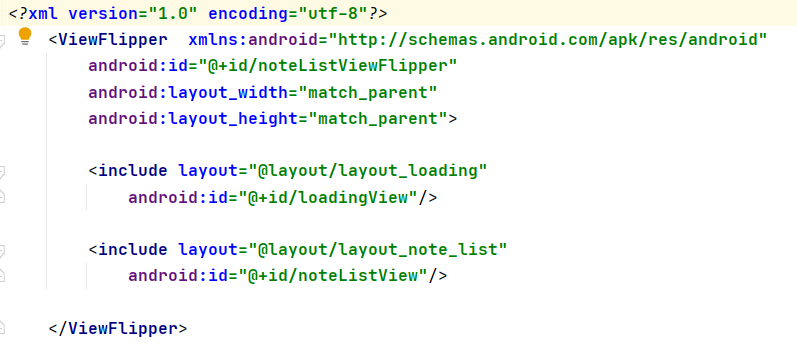
\includegraphics[width=150mm, keepaspectratio]{figures/view_flipper_impl.png}
	\caption{A ViewFlipper komponens használata XML-ben.}
	\label{fig:ViewFlipperComponent}
\end{figure}

\begin{figure}[!ht]
	\centering
	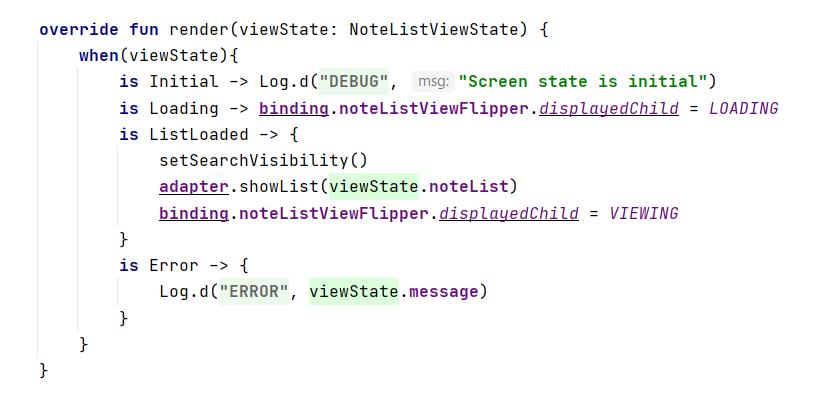
\includegraphics[width=150mm, keepaspectratio]{figures/view_flipper_usage.png}
	\caption{A ViewFlipper megjelenített gyerekének változtatása.}
	\label{fig:ViewFlipperUsage}
\end{figure}

\subsection{Események}
A RainbowCake biztosít keretet arra is, hogyha egyszeri eseményeket szeretnénk a képernyőn megjeleníteni. Ilyen lehet például, ha hibába ütközik az alkalmazás, vagy a visszakapott adatok alapján navigálni szeretnénk egy másik képernyőre. Ezt nem tárolhatjuk az állapotban - hiszen nem olyan dolog, ami minden renderelésnél történik -, ezért megalkották a \emph{OneShotEvent} típust, mely az ilyen eseményeket reprezentálja. \cite{Events}

Használata rendkívül egyszerű, minden lehetséges event típust definiálunk a ViewModelben, majd a megfelelő helyeken a \emph{postEvent} függvénnyel tudjuk elküldeni a fragmentnek, mely az \emph{onEvent} függvény felüldefiniálásával tudja ezeket kezelni. 

\subsection{Tesztelés}
A könyvtár tartalmaz beépített támogatást a ViewModelek és a Presenterek tesztelésére, ezek közül a projekt szempontjából a ViewModel tesztelése releváns. Ennek a fő nehézségét az adja, hogy a beérkezett adatokra állapotváltozás illetve események formájában reagál a ViewModel, melyeket a validáláshoz meg kell figyelnünk valamilyen módon. \cite{RainbowcakeTest}

Ehhez nyújt segítséget az architektúra \emph{ViewModelTest} osztálya. A tesztosztályunkat ebből leszármaztatva elérhetővé válik a \emph{observeStateAndEvents} függvény, mely biztosít egy \emph{stateObserver} és egy \emph{eventsObserver} objektumot. Az előbbi a teszt futása során előforduló \emph{ViewState}-eket figyeli, az utóbbi pedig az eseményeket. Mindkét \emph{observer} tartalmaz \emph{assert} függvényeket az eredmények ellenőrzésére, ilyen például az \emph{assertObserved}, amivel a futás során előforduló összes állapotot vagy eseményt hasonlíthatjuk az elvárthoz, illetve az \emph{assertObservedLast}, mely az előzővel ellentétben csak a legutolsót figyeli. 